
\documentclass[11pt]{article}
\usepackage{amssymb,amsmath,amsthm,latexsym,mathrsfs,array,amssymb,amsmath,epsfig,sudoku,amssymb,amsbsy,array,color,amssymb,amsmath,epsfig,sudoku,url}
\usepackage{minted}
\usepackage{pdflscape}
\usemintedstyle{vs}

\usepackage{amsmath} % For advanced math features like \text, \frac, etc.
\usepackage[utf8]{inputenc} % To handle various characters
\usepackage{float}
\usepackage{booktabs}
%\usepackage[a4paper, margin=0.5in]{geometry}

\textheight 8.5in
\textwidth 6.25in
\voffset= -.55in
\hoffset= -.55in

\date{}
\pagestyle{empty}
\begin{document}
%\begin{landscape}
%\thispagestyle{empty}
\begin{center} {\LARGE\textbf{{CSCI 6360}}}\end{center}
\begin{center}{\Large \textbf{Project 2}}\end{center}
%\begin{center}{Masum Billah \\ University of GA \\ Department of Statistics}\end{center}       
\begin{center} \date{\today} \today \end{center}
    
\vspace{.1in}

\section*{CNN Regression}

\subsection{Architecture}
We utilize a simple CNN architecture consisting of two convolution layers, each followed by an activation function. The output of the final convolution layer is fed into a fully connected layer, which returns the predicted value. The PyTorch implementation of the model is given below.

\begin{minted}{python}
class CNN(nn.Module):
    def __init__(self, n_features, c1=8, c2=16, f=None):
        super().__init__()
        if f is None:
            f = [nn.ReLU, nn.ReLU, nn.ReLU]
            
        self.conv1 = nn.Conv1d(in_channels=1, out_channels=c1, kernel_size=2)
        self.f1 = f[0]()
        self.conv2 = nn.Conv1d(in_channels=c1, out_channels=c2, kernel_size=2)
        self.f2 = f[1]()

        out = c2 * (n_features - 2)
        self.fc1 = nn.Linear(out, 32)
        self.f3 = f[2]()
        self.fc2 = nn.Linear(32, 1)

    def forward(self, x):
        q = self.conv1(x)
        z0 = self.f1(q)
        
        v = self.conv2(z0)
        z1 = self.f2(v)

        z1 = z1.view(z1.size(0), -1)
        
        u = self.fc1(z1)
        z2 = self.f3(u)
        y = self.fc2(z2)
        
        return y
\end{minted}

\subsection{Hyper-parameter Tuning}
To optimize performance, we tuned the model by varying the number of filters, activation functions, learning rates, and mini-batch sizes. Specifically, we evaluated different numbers of filters for Layer 1 and Layer 2: (4, 8), (8, 16), (16, 32), (8, 8), and (16, 16). \\
\\
For activation functions, we evaluated ReLU, Tanh, and their combinations in the CNN layers. We also tested various learning rates to identify which produced the lowest validation Mean Squared Error.\\ 
\\
Finally, we evaluated mini-batch sizes of 2, 4, 8, 16, and 32 to determine the optimum number of samples for gradient approximation. These parameters were individually optimized for each dataset. The Adam optimizer was used in all cases.

%%%%%%%%%%%%%%%%%%%%%%%%%%%%%%%%Auto MPG%%%%%%%%%%%%%%%%%%%%%%%%%%%%%%%%%%%%
\section*{CNN regression on the Auto MPG dataset}
First, the performance of the CNN model for in-sample and validation (80–20 split) was tested using the default parameters with 8 filters in Layer 1 and 16 filters in Layer 2, with ReLU activation in both the CNN and fully connected layers and a learning rate of 0.01. The following table shows the quality of fit of the model.

\begin{table}[H]
\centering
\caption{Auto MPG Dataset: CNN regression performance without fine-tuning.}
\label{tab:Auto_MPG_(In-Sample)}
\begin{tabular}{lrr}
\toprule
 & In-Sample & 80-20 Split \\
\midrule
rSq & 0.882 & 0.880 \\
sst & 23818.994 & 4032.206 \\
sse & 2801.128 & 483.859 \\
mse & 7.146 & 6.125 \\
rmse & 2.673 & 2.475 \\
mae & 1.941 & 1.811 \\
m & 392.000 & 79.000 \\
aic & 5588.874 & 4961.175 \\
bic & 15155.644 & 10669.175 \\
\bottomrule
\end{tabular}
\end{table}

Then, hyperparameter optimization resulted in 8 filters in Layer 1 and 16 filters in Layer 2, with Tanh activation in the CNN layers. The optimal learning rate was 0.02 with a batch size of 2. The following table shows the quality of fit of the tuned model.

\begin{table}[H]
\centering
\caption{Auto MPG dataset: regression performance of the tuned CNN model.}
\label{tab:Auto_MPG_(In-Sample)}
\begin{tabular}{lrr}
\toprule
 & In-Sample & 80-20 Split \\
\midrule
rSq & 0.892 & 0.859 \\
sst & 23818.994 & 4032.206 \\
sse & 2567.609 & 568.952 \\
mse & 6.550 & 7.202 \\
rmse & 2.559 & 2.684 \\
mae & 1.847 & 2.046 \\
m & 392.000 & 79.000 \\
aic & 5554.752 & 4973.974 \\
bic & 15121.522 & 10681.973 \\
\bottomrule
\end{tabular}
\end{table}


\begin{figure}[h]
\centering
\begin{tabular}{cc}
    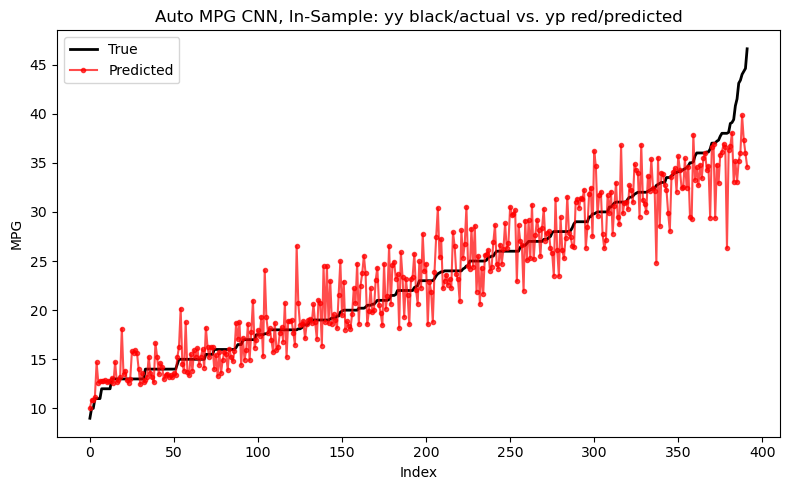
\includegraphics[width=0.5\textwidth]{fig/a1.png} &
    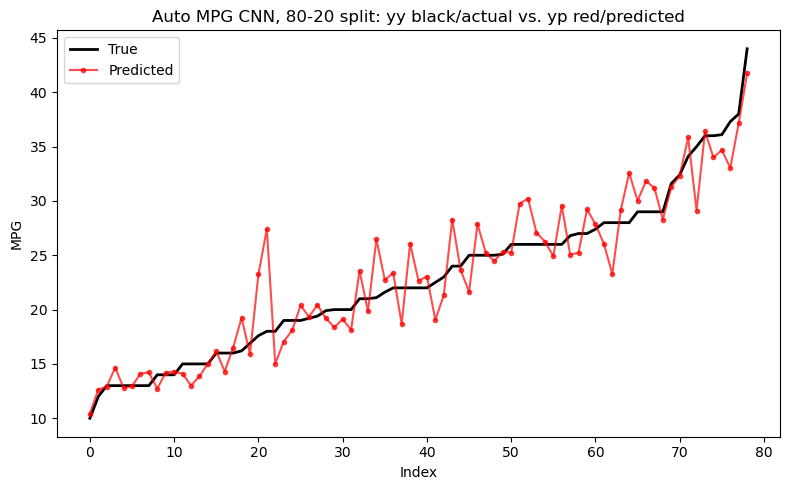
\includegraphics[width=0.5\textwidth]{fig/a2.png} \\
    
    (a) In-sample & (b) Validation (80-20 split)
\end{tabular}
\caption{Performance of the CNN regression on the Auto MPG dataset without fine-tuning.}
\label{fig:cnn1}
\end{figure}

\begin{figure}[h]
\centering

\begin{tabular}{cc}
    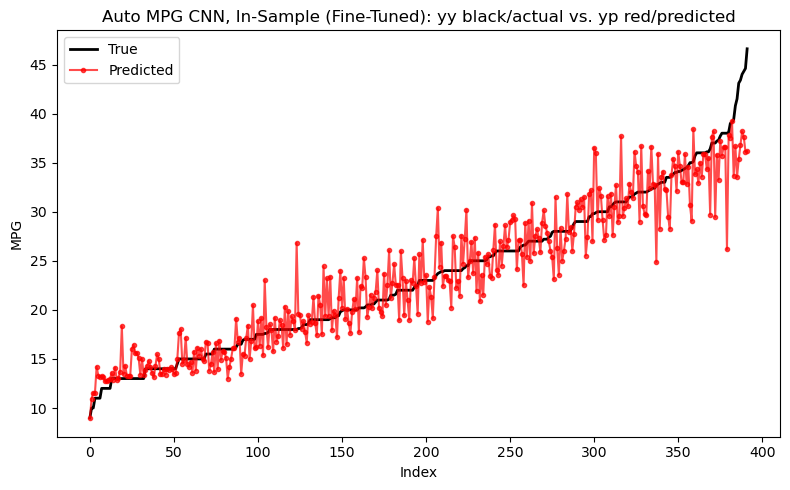
\includegraphics[width=0.5\textwidth]{fig/a3.png} &
    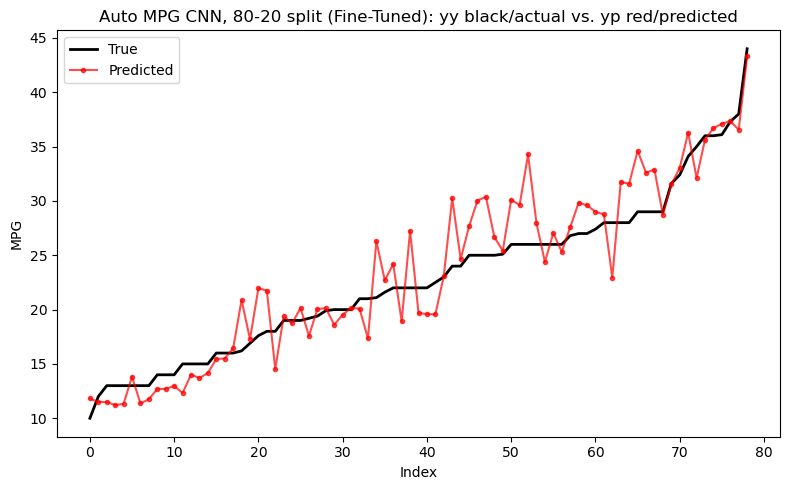
\includegraphics[width=0.5\textwidth]{fig/a4.png} \\
    
    (a) In-sample & (b) Validation (80-20 split)
\end{tabular}

\caption{Performance of the CNN regression model on the Auto MPG dataset with fine-tuning.}
\label{fig:cnn1}
\end{figure}


%%%%%%%%%%%%%%%%%%%%%%%%%%%%%%%%California Housing Price%%%%%%%%%%%%%%%%%%%%%%%%%%%%%%%%%%%%
\section*{CNN regression on the California Housing dataset}
First, the performance of the CNN model for in-sample and validation (80–20 split) was tested using the default parameters with 8 filters in Layer 1 and 16 filters in Layer 2, with ReLU activation in both the CNN and fully connected layers and a learning rate of 0.01. The following table shows the quality of fit of the model.
\begin{table}[H]
\centering
\caption{California Housing: CNN regression performance without fine-tuning.}
\label{tab:California_Housing_(In-Sample)}
\begin{tabular}{lrr}
\toprule
 & In-Sample & 80-20 Split \\
\midrule
rSq & 0.756 & 0.719 \\
sst & 27483.199 & 5409.368 \\
sse & 6719.378 & 1520.702 \\
mse & 0.326 & 0.368 \\
rmse & 0.571 & 0.607 \\
mae & 0.399 & 0.427 \\
m & 20640.000 & 4128.000 \\
aic & -16296.936 & 2743.693 \\
bic & 10943.871 & 24459.300 \\
\bottomrule
\end{tabular}
\end{table}

Then, hyperparameter optimization resulted in 16 filters in Layer 1 and 32 filters in Layer 2, with ReLU activation in the CNN layers. The optimal learning rate was 0.03 with a batch size of 32. The following table shows the quality of fit of the tuned CNN model.

\begin{table}[H]
\centering
\caption{California Housing: regression performance of the tuned CNN model.}
\label{tab:California_Housing_(In-Sample)}
\begin{tabular}{lrr}
\toprule
 & In-Sample & 80-20 Split \\
\midrule
rSq & 0.776 & 0.721 \\
sst & 27483.199 & 5409.368 \\
sse & 6166.594 & 1509.280 \\
mse & 0.299 & 0.366 \\
rmse & 0.547 & 0.605 \\
mae & 0.377 & 0.445 \\
m & 20640.000 & 4128.000 \\
aic & -10308.860 & 10472.570 \\
bic & 47719.694 & 56731.305 \\
\bottomrule
\end{tabular}
\end{table}

\newpage
\begin{figure}[h]
\centering
\begin{tabular}{cc}
    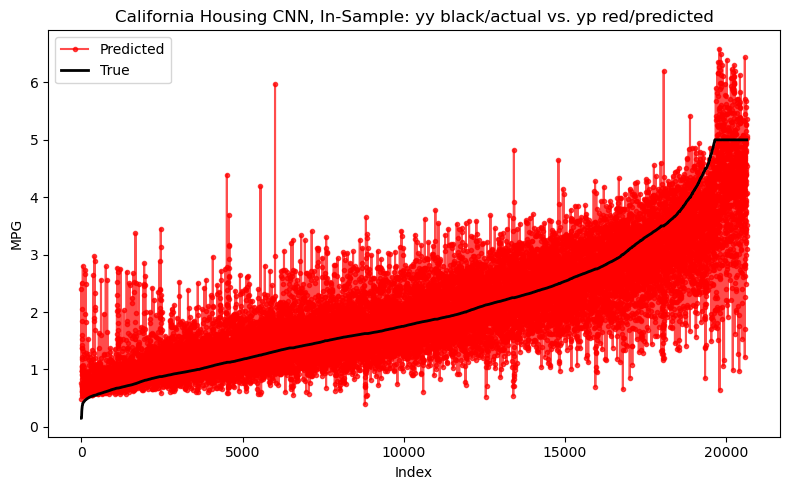
\includegraphics[width=0.5\textwidth]{fig/ch1.png} &
    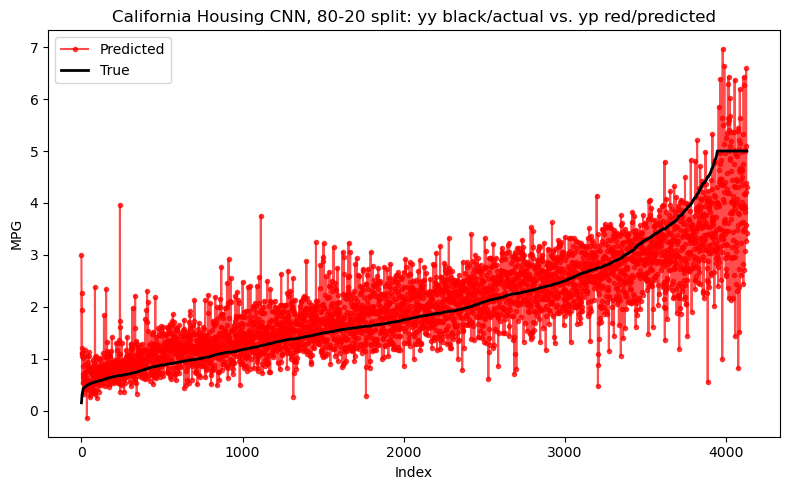
\includegraphics[width=0.5\textwidth]{fig/ch2.png} \\
    
    (a) In-sample & (b) Validation (80-20 split)
\end{tabular}
\caption{Performance of the CNN regression on the California Housing dataset without fine-tuning.}
\label{fig:cnn1}
\end{figure}

\begin{figure}[h]
\centering

\begin{tabular}{cc}
    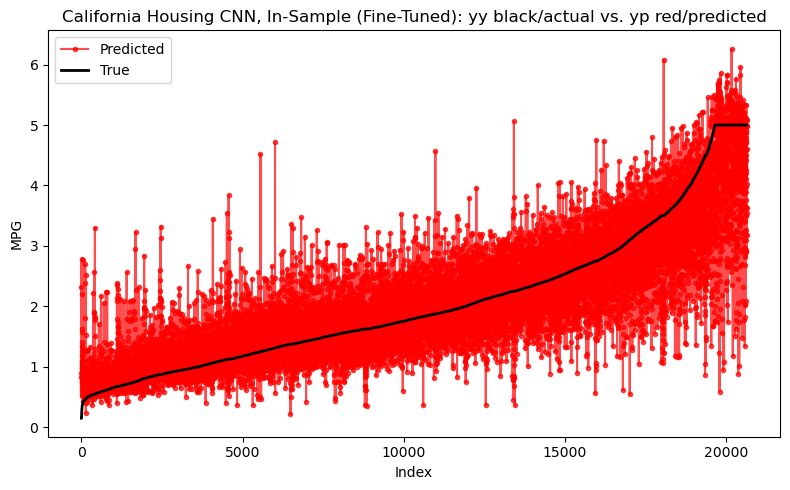
\includegraphics[width=0.5\textwidth]{fig/ch3.png} &
    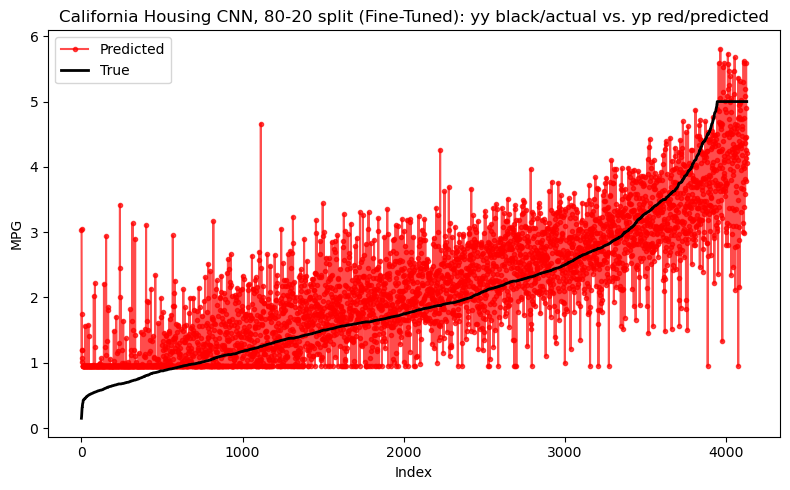
\includegraphics[width=0.5\textwidth]{fig/ch4.png} \\
    
    (a) In-sample & (b) Validation (80-20 split)
\end{tabular}
\caption{Performance of the CNN regression model on the California Housing dataset with fine-tuning.}
\label{fig:cnn1}
\end{figure}
%%%%%%%%%%%%%%%%%%%%%%%%%%%%%%%%Insurance Charges%%%%%%%%%%%%%%%%%%%%%%%%%%%%%%%%%%%%%%%%%%%
\newpage
\section*{CNN regression on the Insurance Charges dataset}
First, the performance of the CNN model for in-sample and validation (80–20 split) was tested using the default parameters with 8 filters in Layer 1 and 16 filters in Layer 2, with ReLU activation in both the CNN and fully connected layers and a learning rate of 0.01. The following table shows the quality of fit of the model.

\begin{table}[H]
\centering
\caption{Insurance Charges: CNN regression performance without fine-tuning.}
\label{tab:Insurance_Charges_(In-Sample)}
\begin{tabular}{lrr}
\toprule
 & In-Sample & 80-20 Split \\
\midrule
rSq & 0.564 & 0.589 \\
sst & 196074242048.000 & 41606660096.000 \\
sse & 85561786368.000 & 17117836288.000 \\
mse & 63947523.444 & 63872523.463 \\
rmse & 7996.720 & 7992.029 \\
mae & 6135.541 & 6441.092 \\
m & 1338.000 & 268.000 \\
aic & 30914.641 & 11682.603 \\
bic & 48762.572 & 24010.461 \\
\bottomrule
\end{tabular}
\end{table}

Then, hyperparameter optimization resulted in 16 filters in Layer 1 and 32 filters in Layer 2, with ReLU activation in the CNN layers. The optimal learning rate was 0.03 with a batch size of 2. The following table shows the quality of fit of the tuned model.

\begin{table}[H]
\centering
\caption{Insurance Charges: regression performance of the tuned CNN model.}
\label{tab:Insurance_Charges_(In-Sample)}
\begin{tabular}{lrr}
\toprule
 & In-Sample & 80-20 Split \\
\midrule
rSq & 0.749 & 0.782 \\
sst & 196074242048.000 & 41606660096.000 \\
sse & 49236451328.000 & 9083892736.000 \\
mse & 36798543.593 & 33895122.149 \\
rmse & 6066.180 & 5821.952 \\
mae & 3993.667 & 3131.384 \\
m & 1338.000 & 268.000 \\
aic & 37935.256 & 19272.793 \\
bic & 75955.040 & 45533.681 \\
\bottomrule
\end{tabular}
\end{table}
\newpage


\begin{figure}[h]
\centering
\begin{tabular}{cc}
    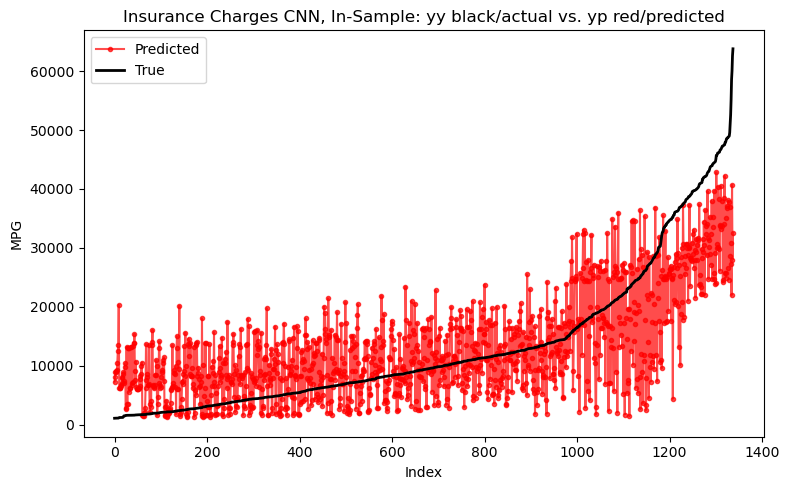
\includegraphics[width=0.5\textwidth]{fig/ins1.png} &
    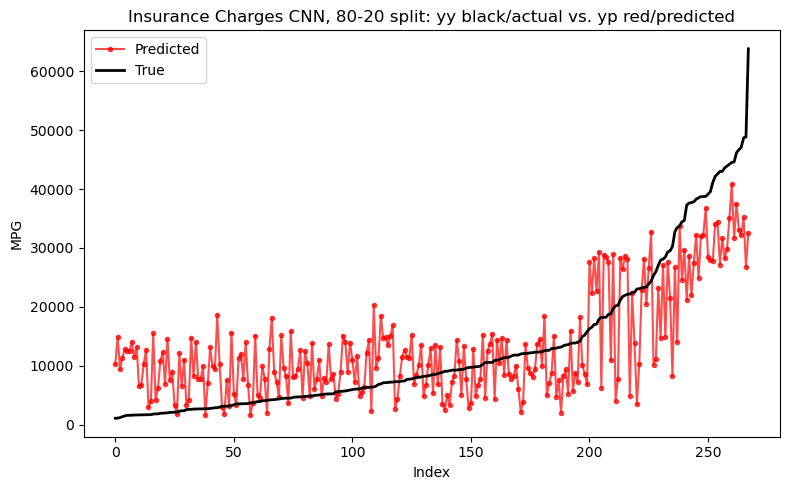
\includegraphics[width=0.5\textwidth]{fig/ins2.png} \\
    
    (a) In-sample & (b) Validation (80-20 split)
\end{tabular}
\caption{Performance of the CNN regression on the Insurance Charges dataset without fine-tuning.}
\label{fig:cnn1}
\end{figure}

\begin{figure}[h]
\centering

\begin{tabular}{cc}
    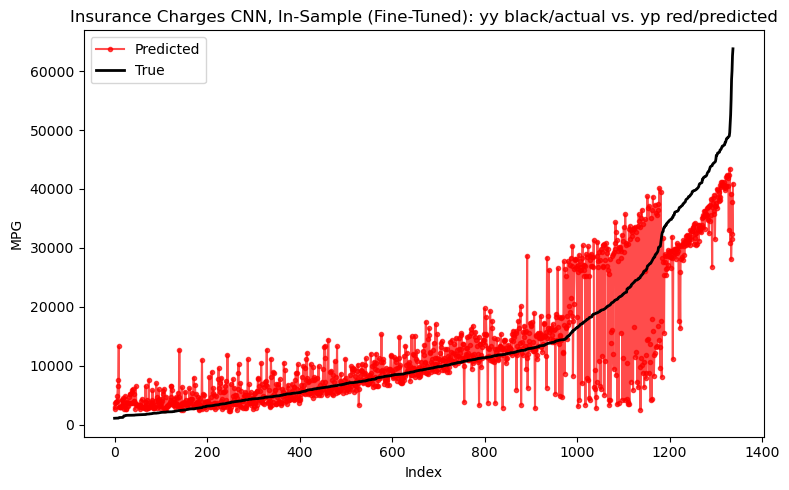
\includegraphics[width=0.5\textwidth]{fig/ins3.png} &
    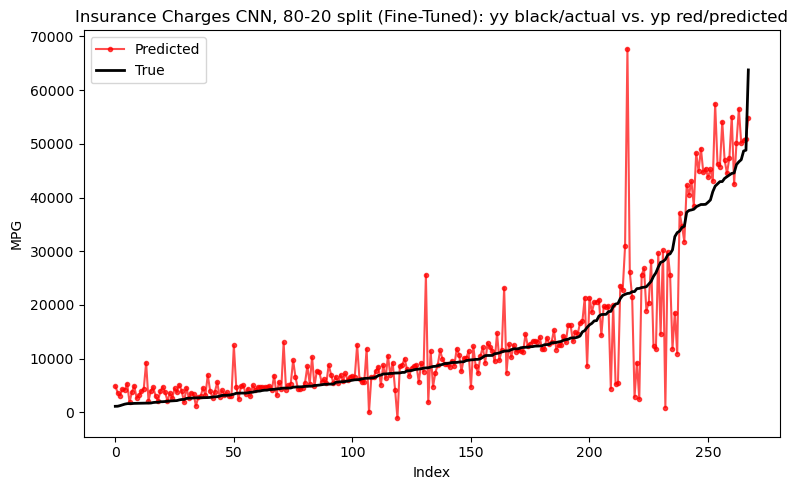
\includegraphics[width=0.5\textwidth]{fig/ins4.png} \\
    
    (a) In-sample & (b) Validation (80-20 split)
\end{tabular}

\caption{Performance of the CNN regression model on the Insurance Charges dataset with fine-tuning.}
\label{fig:cnn1}
\end{figure}


\end{document}